% Created by tikzDevice version 0.12 on 2019-02-08 11:01:06
% !TEX encoding = UTF-8 Unicode
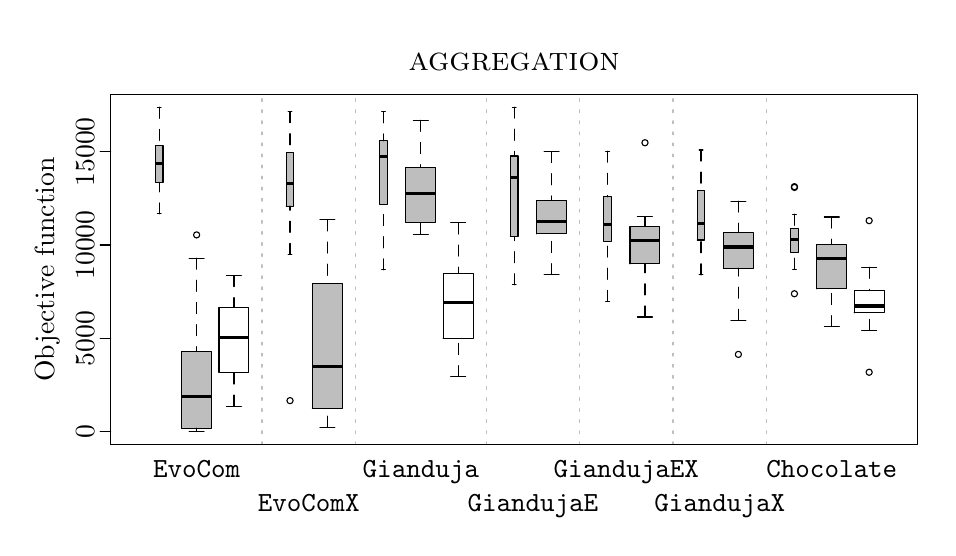
\begin{tikzpicture}[x=1pt,y=1pt]
\definecolor{fillColor}{RGB}{255,255,255}
\path[use as bounding box,fill=fillColor,fill opacity=0.00] (0,0) rectangle (325.21,180.67);
\begin{scope}
\path[clip] ( 30.00, 30.00) rectangle (321.61,156.67);
\definecolor{fillColor}{RGB}{190,190,190}

\path[fill=fillColor] ( 46.20,124.75) --
	( 48.90,124.75) --
	( 48.90,137.93) --
	( 46.20,137.93) --
	cycle;
\definecolor{drawColor}{RGB}{0,0,0}

\path[draw=drawColor,line width= 1.2pt,line join=round] ( 46.20,131.70) -- ( 48.90,131.70);

\path[draw=drawColor,line width= 0.4pt,dash pattern=on 4pt off 4pt ,line join=round,line cap=round] ( 47.55,113.38) -- ( 47.55,124.75);

\path[draw=drawColor,line width= 0.4pt,dash pattern=on 4pt off 4pt ,line join=round,line cap=round] ( 47.55,151.91) -- ( 47.55,137.93);

\path[draw=drawColor,line width= 0.4pt,line join=round,line cap=round] ( 46.88,113.38) -- ( 48.23,113.38);

\path[draw=drawColor,line width= 0.4pt,line join=round,line cap=round] ( 46.88,151.91) -- ( 48.23,151.91);

\path[draw=drawColor,line width= 0.4pt,line join=round,line cap=round] ( 46.20,124.75) --
	( 48.90,124.75) --
	( 48.90,137.93) --
	( 46.20,137.93) --
	( 46.20,124.75);

\path[fill=fillColor] ( 55.65, 35.96) --
	( 66.45, 35.96) --
	( 66.45, 63.62) --
	( 55.65, 63.62) --
	cycle;

\path[draw=drawColor,line width= 1.2pt,line join=round] ( 55.65, 47.47) -- ( 66.45, 47.47);

\path[draw=drawColor,line width= 0.4pt,dash pattern=on 4pt off 4pt ,line join=round,line cap=round] ( 61.05, 34.69) -- ( 61.05, 35.96);

\path[draw=drawColor,line width= 0.4pt,dash pattern=on 4pt off 4pt ,line join=round,line cap=round] ( 61.05, 97.39) -- ( 61.05, 63.62);

\path[draw=drawColor,line width= 0.4pt,line join=round,line cap=round] ( 58.35, 34.69) -- ( 63.75, 34.69);

\path[draw=drawColor,line width= 0.4pt,line join=round,line cap=round] ( 58.35, 97.39) -- ( 63.75, 97.39);

\path[draw=drawColor,line width= 0.4pt,line join=round,line cap=round] ( 55.65, 35.96) --
	( 66.45, 35.96) --
	( 66.45, 63.62) --
	( 55.65, 63.62) --
	( 55.65, 35.96);

\path[draw=drawColor,line width= 0.4pt,line join=round,line cap=round] ( 61.05,105.79) circle (  1.12);
\definecolor{fillColor}{RGB}{255,255,255}

\path[fill=fillColor] ( 69.15, 56.09) --
	( 79.95, 56.09) --
	( 79.95, 79.69) --
	( 69.15, 79.69) --
	cycle;

\path[draw=drawColor,line width= 1.2pt,line join=round] ( 69.15, 68.68) -- ( 79.95, 68.68);

\path[draw=drawColor,line width= 0.4pt,dash pattern=on 4pt off 4pt ,line join=round,line cap=round] ( 74.55, 43.91) -- ( 74.55, 56.09);

\path[draw=drawColor,line width= 0.4pt,dash pattern=on 4pt off 4pt ,line join=round,line cap=round] ( 74.55, 91.11) -- ( 74.55, 79.69);

\path[draw=drawColor,line width= 0.4pt,line join=round,line cap=round] ( 71.85, 43.91) -- ( 77.25, 43.91);

\path[draw=drawColor,line width= 0.4pt,line join=round,line cap=round] ( 71.85, 91.11) -- ( 77.25, 91.11);

\path[draw=drawColor,line width= 0.4pt,line join=round,line cap=round] ( 69.15, 56.09) --
	( 79.95, 56.09) --
	( 79.95, 79.69) --
	( 69.15, 79.69) --
	( 69.15, 56.09);
\definecolor{fillColor}{RGB}{190,190,190}

\path[fill=fillColor] ( 93.45,116.18) --
	( 96.15,116.18) --
	( 96.15,135.65) --
	( 93.45,135.65) --
	cycle;

\path[draw=drawColor,line width= 1.2pt,line join=round] ( 93.45,124.38) -- ( 96.15,124.38);

\path[draw=drawColor,line width= 0.4pt,dash pattern=on 4pt off 4pt ,line join=round,line cap=round] ( 94.80, 98.71) -- ( 94.80,116.18);

\path[draw=drawColor,line width= 0.4pt,dash pattern=on 4pt off 4pt ,line join=round,line cap=round] ( 94.80,150.34) -- ( 94.80,135.65);

\path[draw=drawColor,line width= 0.4pt,line join=round,line cap=round] ( 94.13, 98.71) -- ( 95.48, 98.71);

\path[draw=drawColor,line width= 0.4pt,line join=round,line cap=round] ( 94.13,150.34) -- ( 95.48,150.34);

\path[draw=drawColor,line width= 0.4pt,line join=round,line cap=round] ( 93.45,116.18) --
	( 96.15,116.18) --
	( 96.15,135.65) --
	( 93.45,135.65) --
	( 93.45,116.18);

\path[draw=drawColor,line width= 0.4pt,line join=round,line cap=round] ( 94.80, 45.90) circle (  1.12);

\path[fill=fillColor] (102.90, 43.20) --
	(113.70, 43.20) --
	(113.70, 88.11) --
	(102.90, 88.11) --
	cycle;

\path[draw=drawColor,line width= 1.2pt,line join=round] (102.90, 58.28) -- (113.70, 58.28);

\path[draw=drawColor,line width= 0.4pt,dash pattern=on 4pt off 4pt ,line join=round,line cap=round] (108.30, 36.32) -- (108.30, 43.20);

\path[draw=drawColor,line width= 0.4pt,dash pattern=on 4pt off 4pt ,line join=round,line cap=round] (108.30,111.21) -- (108.30, 88.11);

\path[draw=drawColor,line width= 0.4pt,line join=round,line cap=round] (105.60, 36.32) -- (111.00, 36.32);

\path[draw=drawColor,line width= 0.4pt,line join=round,line cap=round] (105.60,111.21) -- (111.00,111.21);

\path[draw=drawColor,line width= 0.4pt,line join=round,line cap=round] (102.90, 43.20) --
	(113.70, 43.20) --
	(113.70, 88.11) --
	(102.90, 88.11) --
	(102.90, 43.20);

\path[fill=fillColor] (127.20,116.89) --
	(129.91,116.89) --
	(129.91,139.80) --
	(127.20,139.80) --
	cycle;

\path[draw=drawColor,line width= 1.2pt,line join=round] (127.20,134.16) -- (129.91,134.16);

\path[draw=drawColor,line width= 0.4pt,dash pattern=on 4pt off 4pt ,line join=round,line cap=round] (128.56, 93.15) -- (128.56,116.89);

\path[draw=drawColor,line width= 0.4pt,dash pattern=on 4pt off 4pt ,line join=round,line cap=round] (128.56,150.31) -- (128.56,139.80);

\path[draw=drawColor,line width= 0.4pt,line join=round,line cap=round] (127.88, 93.15) -- (129.23, 93.15);

\path[draw=drawColor,line width= 0.4pt,line join=round,line cap=round] (127.88,150.31) -- (129.23,150.31);

\path[draw=drawColor,line width= 0.4pt,line join=round,line cap=round] (127.20,116.89) --
	(129.91,116.89) --
	(129.91,139.80) --
	(127.20,139.80) --
	(127.20,116.89);

\path[fill=fillColor] (136.66,110.33) --
	(147.46,110.33) --
	(147.46,130.24) --
	(136.66,130.24) --
	cycle;

\path[draw=drawColor,line width= 1.2pt,line join=round] (136.66,120.69) -- (147.46,120.69);

\path[draw=drawColor,line width= 0.4pt,dash pattern=on 4pt off 4pt ,line join=round,line cap=round] (142.06,106.06) -- (142.06,110.33);

\path[draw=drawColor,line width= 0.4pt,dash pattern=on 4pt off 4pt ,line join=round,line cap=round] (142.06,147.20) -- (142.06,130.24);

\path[draw=drawColor,line width= 0.4pt,line join=round,line cap=round] (139.36,106.06) -- (144.76,106.06);

\path[draw=drawColor,line width= 0.4pt,line join=round,line cap=round] (139.36,147.20) -- (144.76,147.20);

\path[draw=drawColor,line width= 0.4pt,line join=round,line cap=round] (136.66,110.33) --
	(147.46,110.33) --
	(147.46,130.24) --
	(136.66,130.24) --
	(136.66,110.33);
\definecolor{fillColor}{RGB}{255,255,255}

\path[fill=fillColor] (150.16, 68.40) --
	(160.96, 68.40) --
	(160.96, 91.88) --
	(150.16, 91.88) --
	cycle;

\path[draw=drawColor,line width= 1.2pt,line join=round] (150.16, 81.37) -- (160.96, 81.37);

\path[draw=drawColor,line width= 0.4pt,dash pattern=on 4pt off 4pt ,line join=round,line cap=round] (155.56, 54.56) -- (155.56, 68.40);

\path[draw=drawColor,line width= 0.4pt,dash pattern=on 4pt off 4pt ,line join=round,line cap=round] (155.56,110.12) -- (155.56, 91.88);

\path[draw=drawColor,line width= 0.4pt,line join=round,line cap=round] (152.86, 54.56) -- (158.26, 54.56);

\path[draw=drawColor,line width= 0.4pt,line join=round,line cap=round] (152.86,110.12) -- (158.26,110.12);

\path[draw=drawColor,line width= 0.4pt,line join=round,line cap=round] (150.16, 68.40) --
	(160.96, 68.40) --
	(160.96, 91.88) --
	(150.16, 91.88) --
	(150.16, 68.40);
\definecolor{fillColor}{RGB}{190,190,190}

\path[fill=fillColor] (174.46,105.19) --
	(177.16,105.19) --
	(177.16,134.29) --
	(174.46,134.29) --
	cycle;

\path[draw=drawColor,line width= 1.2pt,line join=round] (174.46,126.50) -- (177.16,126.50);

\path[draw=drawColor,line width= 0.4pt,dash pattern=on 4pt off 4pt ,line join=round,line cap=round] (175.81, 87.74) -- (175.81,105.19);

\path[draw=drawColor,line width= 0.4pt,dash pattern=on 4pt off 4pt ,line join=round,line cap=round] (175.81,151.98) -- (175.81,134.29);

\path[draw=drawColor,line width= 0.4pt,line join=round,line cap=round] (175.13, 87.74) -- (176.48, 87.74);

\path[draw=drawColor,line width= 0.4pt,line join=round,line cap=round] (175.13,151.98) -- (176.48,151.98);

\path[draw=drawColor,line width= 0.4pt,line join=round,line cap=round] (174.46,105.19) --
	(177.16,105.19) --
	(177.16,134.29) --
	(174.46,134.29) --
	(174.46,105.19);

\path[fill=fillColor] (183.91,106.14) --
	(194.71,106.14) --
	(194.71,118.36) --
	(183.91,118.36) --
	cycle;

\path[draw=drawColor,line width= 1.2pt,line join=round] (183.91,110.64) -- (194.71,110.64);

\path[draw=drawColor,line width= 0.4pt,dash pattern=on 4pt off 4pt ,line join=round,line cap=round] (189.31, 91.41) -- (189.31,106.14);

\path[draw=drawColor,line width= 0.4pt,dash pattern=on 4pt off 4pt ,line join=round,line cap=round] (189.31,135.89) -- (189.31,118.36);

\path[draw=drawColor,line width= 0.4pt,line join=round,line cap=round] (186.61, 91.41) -- (192.01, 91.41);

\path[draw=drawColor,line width= 0.4pt,line join=round,line cap=round] (186.61,135.89) -- (192.01,135.89);

\path[draw=drawColor,line width= 0.4pt,line join=round,line cap=round] (183.91,106.14) --
	(194.71,106.14) --
	(194.71,118.36) --
	(183.91,118.36) --
	(183.91,106.14);

\path[fill=fillColor] (208.21,103.47) --
	(210.91,103.47) --
	(210.91,119.55) --
	(208.21,119.55) --
	cycle;

\path[draw=drawColor,line width= 1.2pt,line join=round] (208.21,109.65) -- (210.91,109.65);

\path[draw=drawColor,line width= 0.4pt,dash pattern=on 4pt off 4pt ,line join=round,line cap=round] (209.56, 81.74) -- (209.56,103.47);

\path[draw=drawColor,line width= 0.4pt,dash pattern=on 4pt off 4pt ,line join=round,line cap=round] (209.56,136.05) -- (209.56,119.55);

\path[draw=drawColor,line width= 0.4pt,line join=round,line cap=round] (208.88, 81.74) -- (210.23, 81.74);

\path[draw=drawColor,line width= 0.4pt,line join=round,line cap=round] (208.88,136.05) -- (210.23,136.05);

\path[draw=drawColor,line width= 0.4pt,line join=round,line cap=round] (208.21,103.47) --
	(210.91,103.47) --
	(210.91,119.55) --
	(208.21,119.55) --
	(208.21,103.47);

\path[fill=fillColor] (217.66, 95.37) --
	(228.46, 95.37) --
	(228.46,108.86) --
	(217.66,108.86) --
	cycle;

\path[draw=drawColor,line width= 1.2pt,line join=round] (217.66,103.70) -- (228.46,103.70);

\path[draw=drawColor,line width= 0.4pt,dash pattern=on 4pt off 4pt ,line join=round,line cap=round] (223.06, 76.11) -- (223.06, 95.37);

\path[draw=drawColor,line width= 0.4pt,dash pattern=on 4pt off 4pt ,line join=round,line cap=round] (223.06,112.42) -- (223.06,108.86);

\path[draw=drawColor,line width= 0.4pt,line join=round,line cap=round] (220.36, 76.11) -- (225.76, 76.11);

\path[draw=drawColor,line width= 0.4pt,line join=round,line cap=round] (220.36,112.42) -- (225.76,112.42);

\path[draw=drawColor,line width= 0.4pt,line join=round,line cap=round] (217.66, 95.37) --
	(228.46, 95.37) --
	(228.46,108.86) --
	(217.66,108.86) --
	(217.66, 95.37);

\path[draw=drawColor,line width= 0.4pt,line join=round,line cap=round] (223.06,139.09) circle (  1.12);

\path[fill=fillColor] (241.96,103.93) --
	(244.66,103.93) --
	(244.66,121.92) --
	(241.96,121.92) --
	cycle;

\path[draw=drawColor,line width= 1.2pt,line join=round] (241.96,109.96) -- (244.66,109.96);

\path[draw=drawColor,line width= 0.4pt,dash pattern=on 4pt off 4pt ,line join=round,line cap=round] (243.31, 91.33) -- (243.31,103.93);

\path[draw=drawColor,line width= 0.4pt,dash pattern=on 4pt off 4pt ,line join=round,line cap=round] (243.31,136.47) -- (243.31,121.92);

\path[draw=drawColor,line width= 0.4pt,line join=round,line cap=round] (242.64, 91.33) -- (243.99, 91.33);

\path[draw=drawColor,line width= 0.4pt,line join=round,line cap=round] (242.64,136.47) -- (243.99,136.47);

\path[draw=drawColor,line width= 0.4pt,line join=round,line cap=round] (241.96,103.93) --
	(244.66,103.93) --
	(244.66,121.92) --
	(241.96,121.92) --
	(241.96,103.93);

\path[fill=fillColor] (251.41, 93.75) --
	(262.21, 93.75) --
	(262.21,106.66) --
	(251.41,106.66) --
	cycle;

\path[draw=drawColor,line width= 1.2pt,line join=round] (251.41,101.47) -- (262.21,101.47);

\path[draw=drawColor,line width= 0.4pt,dash pattern=on 4pt off 4pt ,line join=round,line cap=round] (256.81, 74.91) -- (256.81, 93.75);

\path[draw=drawColor,line width= 0.4pt,dash pattern=on 4pt off 4pt ,line join=round,line cap=round] (256.81,118.01) -- (256.81,106.66);

\path[draw=drawColor,line width= 0.4pt,line join=round,line cap=round] (254.11, 74.91) -- (259.51, 74.91);

\path[draw=drawColor,line width= 0.4pt,line join=round,line cap=round] (254.11,118.01) -- (259.51,118.01);

\path[draw=drawColor,line width= 0.4pt,line join=round,line cap=round] (251.41, 93.75) --
	(262.21, 93.75) --
	(262.21,106.66) --
	(251.41,106.66) --
	(251.41, 93.75);

\path[draw=drawColor,line width= 0.4pt,line join=round,line cap=round] (256.81, 62.61) circle (  1.12);

\path[fill=fillColor] (275.71, 99.58) --
	(278.41, 99.58) --
	(278.41,108.25) --
	(275.71,108.25) --
	cycle;

\path[draw=drawColor,line width= 1.2pt,line join=round] (275.71,104.24) -- (278.41,104.24);

\path[draw=drawColor,line width= 0.4pt,dash pattern=on 4pt off 4pt ,line join=round,line cap=round] (277.06, 93.37) -- (277.06, 99.58);

\path[draw=drawColor,line width= 0.4pt,dash pattern=on 4pt off 4pt ,line join=round,line cap=round] (277.06,113.25) -- (277.06,108.25);

\path[draw=drawColor,line width= 0.4pt,line join=round,line cap=round] (276.39, 93.37) -- (277.74, 93.37);

\path[draw=drawColor,line width= 0.4pt,line join=round,line cap=round] (276.39,113.25) -- (277.74,113.25);

\path[draw=drawColor,line width= 0.4pt,line join=round,line cap=round] (275.71, 99.58) --
	(278.41, 99.58) --
	(278.41,108.25) --
	(275.71,108.25) --
	(275.71, 99.58);

\path[draw=drawColor,line width= 0.4pt,line join=round,line cap=round] (277.06, 84.53) circle (  1.12);

\path[draw=drawColor,line width= 0.4pt,line join=round,line cap=round] (277.06,123.22) circle (  1.12);

\path[draw=drawColor,line width= 0.4pt,line join=round,line cap=round] (277.06,122.94) circle (  1.12);

\path[fill=fillColor] (285.16, 86.26) --
	(295.96, 86.26) --
	(295.96,102.29) --
	(285.16,102.29) --
	cycle;

\path[draw=drawColor,line width= 1.2pt,line join=round] (285.16, 97.24) -- (295.96, 97.24);

\path[draw=drawColor,line width= 0.4pt,dash pattern=on 4pt off 4pt ,line join=round,line cap=round] (290.56, 72.63) -- (290.56, 86.26);

\path[draw=drawColor,line width= 0.4pt,dash pattern=on 4pt off 4pt ,line join=round,line cap=round] (290.56,112.24) -- (290.56,102.29);

\path[draw=drawColor,line width= 0.4pt,line join=round,line cap=round] (287.86, 72.63) -- (293.26, 72.63);

\path[draw=drawColor,line width= 0.4pt,line join=round,line cap=round] (287.86,112.24) -- (293.26,112.24);

\path[draw=drawColor,line width= 0.4pt,line join=round,line cap=round] (285.16, 86.26) --
	(295.96, 86.26) --
	(295.96,102.29) --
	(285.16,102.29) --
	(285.16, 86.26);
\definecolor{fillColor}{RGB}{255,255,255}

\path[fill=fillColor] (298.66, 77.66) --
	(309.46, 77.66) --
	(309.46, 85.66) --
	(298.66, 85.66) --
	cycle;

\path[draw=drawColor,line width= 1.2pt,line join=round] (298.66, 80.14) -- (309.46, 80.14);

\path[draw=drawColor,line width= 0.4pt,dash pattern=on 4pt off 4pt ,line join=round,line cap=round] (304.06, 71.28) -- (304.06, 77.66);

\path[draw=drawColor,line width= 0.4pt,dash pattern=on 4pt off 4pt ,line join=round,line cap=round] (304.06, 94.09) -- (304.06, 85.66);

\path[draw=drawColor,line width= 0.4pt,line join=round,line cap=round] (301.36, 71.28) -- (306.76, 71.28);

\path[draw=drawColor,line width= 0.4pt,line join=round,line cap=round] (301.36, 94.09) -- (306.76, 94.09);

\path[draw=drawColor,line width= 0.4pt,line join=round,line cap=round] (298.66, 77.66) --
	(309.46, 77.66) --
	(309.46, 85.66) --
	(298.66, 85.66) --
	(298.66, 77.66);

\path[draw=drawColor,line width= 0.4pt,line join=round,line cap=round] (304.06, 56.16) circle (  1.12);

\path[draw=drawColor,line width= 0.4pt,line join=round,line cap=round] (304.06,110.93) circle (  1.12);
\definecolor{drawColor}{RGB}{190,190,190}

\path[draw=drawColor,line width= 0.4pt,dash pattern=on 1pt off 3pt ,line join=round,line cap=round] ( 84.68, 30.00) -- ( 84.68,156.67);

\path[draw=drawColor,line width= 0.4pt,dash pattern=on 1pt off 3pt ,line join=round,line cap=round] (118.43, 30.00) -- (118.43,156.67);

\path[draw=drawColor,line width= 0.4pt,dash pattern=on 1pt off 3pt ,line join=round,line cap=round] (165.68, 30.00) -- (165.68,156.67);

\path[draw=drawColor,line width= 0.4pt,dash pattern=on 1pt off 3pt ,line join=round,line cap=round] (199.43, 30.00) -- (199.43,156.67);

\path[draw=drawColor,line width= 0.4pt,dash pattern=on 1pt off 3pt ,line join=round,line cap=round] (233.19, 30.00) -- (233.19,156.67);

\path[draw=drawColor,line width= 0.4pt,dash pattern=on 1pt off 3pt ,line join=round,line cap=round] (266.94, 30.00) -- (266.94,156.67);
\end{scope}
\begin{scope}
\path[clip] (  0.00,  0.00) rectangle (325.21,180.67);
\definecolor{drawColor}{RGB}{0,0,0}

\node[text=drawColor,anchor=base,inner sep=0pt, outer sep=0pt, scale=  1.00] at ( 61.05, 18.00) {\texttt{EvoCom}};

\node[text=drawColor,anchor=base,inner sep=0pt, outer sep=0pt, scale=  1.00] at (142.06, 18.00) {\texttt{Gianduja}};

\node[text=drawColor,anchor=base,inner sep=0pt, outer sep=0pt, scale=  1.00] at (216.31, 18.00) {\texttt{GiandujaEX}};

\node[text=drawColor,anchor=base,inner sep=0pt, outer sep=0pt, scale=  1.00] at (290.56, 18.00) {\texttt{Chocolate}};

\node[text=drawColor,anchor=base,inner sep=0pt, outer sep=0pt, scale=  1.00] at (101.55,  6.00) {\texttt{EvoComX}};

\node[text=drawColor,anchor=base,inner sep=0pt, outer sep=0pt, scale=  1.00] at (182.56,  6.00) {\texttt{GiandujaE}};

\node[text=drawColor,anchor=base,inner sep=0pt, outer sep=0pt, scale=  1.00] at (250.06,  6.00) {\texttt{GiandujaX}};
\end{scope}
\begin{scope}
\path[clip] (  0.00,  0.00) rectangle (325.21,180.67);
\definecolor{drawColor}{RGB}{0,0,0}

\node[text=drawColor,anchor=base,inner sep=0pt, outer sep=0pt, scale=  1.20] at (175.81,165.07) {\textsc{aggregation}};

\node[text=drawColor,rotate= 90.00,anchor=base,inner sep=0pt, outer sep=0pt, scale=  1.00] at (  9.60, 93.34) {Objective function};
\end{scope}
\begin{scope}
\path[clip] (  0.00,  0.00) rectangle (325.21,180.67);
\definecolor{drawColor}{RGB}{0,0,0}

\path[draw=drawColor,line width= 0.4pt,line join=round,line cap=round] ( 30.00, 34.69) -- ( 30.00,135.83);

\path[draw=drawColor,line width= 0.4pt,line join=round,line cap=round] ( 30.00, 34.69) -- ( 26.20, 34.69);

\path[draw=drawColor,line width= 0.4pt,line join=round,line cap=round] ( 30.00, 68.41) -- ( 26.20, 68.41);

\path[draw=drawColor,line width= 0.4pt,line join=round,line cap=round] ( 30.00,102.12) -- ( 26.20,102.12);

\path[draw=drawColor,line width= 0.4pt,line join=round,line cap=round] ( 30.00,135.83) -- ( 26.20,135.83);

\node[text=drawColor,rotate= 90.00,anchor=base,inner sep=0pt, outer sep=0pt, scale=  1.00] at ( 24.00, 34.69) {0};

\node[text=drawColor,rotate= 90.00,anchor=base,inner sep=0pt, outer sep=0pt, scale=  1.00] at ( 24.00, 68.41) {5000};

\node[text=drawColor,rotate= 90.00,anchor=base,inner sep=0pt, outer sep=0pt, scale=  1.00] at ( 24.00,102.12) {10000};

\node[text=drawColor,rotate= 90.00,anchor=base,inner sep=0pt, outer sep=0pt, scale=  1.00] at ( 24.00,135.83) {15000};

\path[draw=drawColor,line width= 0.4pt,line join=round,line cap=round] ( 30.00, 30.00) --
	(321.61, 30.00) --
	(321.61,156.67) --
	( 30.00,156.67) --
	( 30.00, 30.00);
\end{scope}
\end{tikzpicture}
